% y = arch(x)
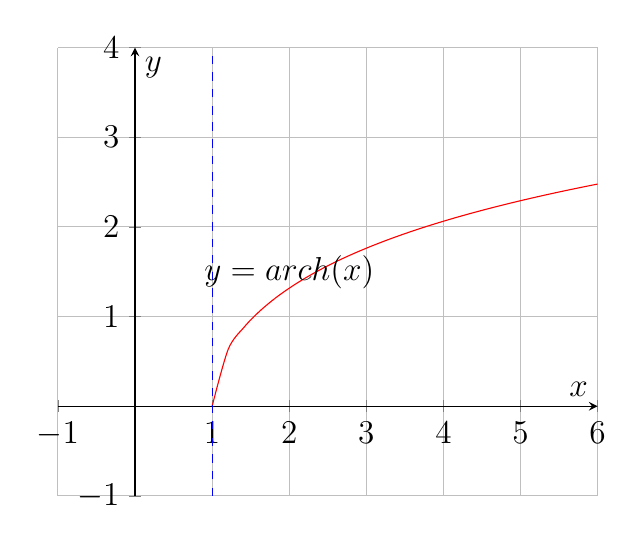
\begin{tikzpicture}
  \begin{axis}[xmin=-1, xmax=6,ymin=-1,ymax=4, grid=both, font=\large, axis lines = middle,
    smooth, xlabel={$x$}, ylabel={$y$}]
    \addplot[draw=red,domain=1:6] {ln(x + sqrt(x^2 - 1))};
    \addplot[dashed, draw=blue, mark=none] coordinates {(1, -1) (1, 4)};
    \node at (axis cs:2,1.5) {$y = arch(x)$};
  \end{axis}
\end{tikzpicture}
